\hypertarget{acknowledgements}{%
\chapter*{Acknowledgements}\label{acknowledgements}}
\addcontentsline{toc}{chapter}{Acknowledgements}

\hypertarget{summary}{%
\chapter*{Summary}\label{summary}}
\addcontentsline{toc}{chapter}{Summary}

\hypertarget{samenvatting}{%
\chapter*{Samenvatting}\label{samenvatting}}
\addcontentsline{toc}{chapter}{Samenvatting}

\mainmatter

\hypertarget{introduction}{%
\chapter{Introduction}\label{introduction}}

\hypertarget{unipept-desktop-a-faster-more-powerful-metaproteomics-results-analysis-tool}{%
\chapter{Unipept Desktop: a faster, more powerful metaproteomics results
analysis
tool}\label{unipept-desktop-a-faster-more-powerful-metaproteomics-results-analysis-tool}}

\textbf{Abstract} Metaproteomics has become an important research tool
to study microbial systems, which has resulted in increased
metaproteomics data generation. However, efficient tools for processing
the acquired data have lagged behind. One widely used tool for
metaproteomics data interpretation is Unipept, a web-based tool that
provides, amongst others, interactive and insightful visualizations. Due
to its web-based implementation, however, the Unipept web application is
limited in the amount of data that can be analyzed. In this manuscript
we therefore present Unipept Desktop, a desktop application version of
Unipept that is designed to drastically increase the throughput and
capacity of metaproteomics data analysis. Moreover, it provides a novel
comparative analysis pipeline and improves the organization of
experimental data into projects, thus addressing the growing need for
more performant and versatile analysis tools for metaproteomics data.

\hypertarget{introduction-1}{%
\section{Introduction}\label{introduction-1}}

Metaproteomics is a relatively young research field that focuses on the
study of microbial environments and complex ecosystems, and of the
interactions between the organisms involved, through the analysis of the
proteins extracted from these environments. Over the past years, the
technology to identify proteins from such complex samples has been
greatly improved, allowing metaproteomics to transition from relatively
small studies to large scale experiments. The key enabling technologies
for this transition are improved mass spectrometers and more powerful
proteomics approaches, which have both come a long way since the
introduction of metaproteomics analysis in 2004. To allow efficient
processing of the resulting increase of acquired data, various dedicated
tools have been made available to support metaproteomics data analysis,
but even with this increased bioinformatics support, many challenges
still need to be overcome, especially regarding downstream analysis of
the obtained identifications.

Unipept is a leading tool for such downstream metaproteomics data
analysis that currently consists of a web application, a web service,
and a command line tool. The Unipept web application provides users with
the ability to analyze a metaproteomics sample and extract taxonomic and
functional information from environmental samples derived from a variety
of origins, ranging from the human gut to biogas plants. The Unipept web
application provides users with interactive visualizations and allows
them to, for example, filter out all functions that are associated with
a specific taxon. Due to its web-based nature, however, the size and
number of samples that can be analyzed by Unipept are limited. And while
it is currently possible to analyze larger data sets using the Unipept
CLI, this requires more sophisticated bioinformatics skills and does not
provide the interactive link between taxa and functional annotations.

Because of the browser limitations, it can already take a substantial
amount of time to process relatively small samples (e.g.~containing up
to a few thousand identified peptides) using Unipept, depending on the
specific search configuration used. These limitations have become an
issue, as the advances in metaproteomics have not only increased data
set sizes, but have also increased the number of data sets that need to
be processed.

In order to accommodate this evolution, the throughput of metaproteomics
data analyses needs to increase as well, in turn requiring tools that
are not constrained in the amount of memory and CPU resources they are
allowed to consume. Moreover, analysis results also need to be retained
for future reference, ideally in a project-based approach that can group
multiple samples, and the corresponding results should be easily
shareable with other researchers.

For specific applications, it is also important that all data is
processed offline or on-site rather than being sent over the internet.
For instance, sensitive medical data is often not allowed to be sent to
external services for processing, but must be kept in-house to safeguard
patient confidentiality and privacy.

All of the above issues need to be resolved in order to support the
growing interest in, and reach of, metaproteomics. We therefore here
present the Unipept Desktop Application, a novel cross-platform desktop
application designed to specifically overcome these challenges while
also retaining the functionality that exists in the current web app.

\hypertarget{implementation}{%
\section{Implementation}\label{implementation}}

\begin{figure}
\centering
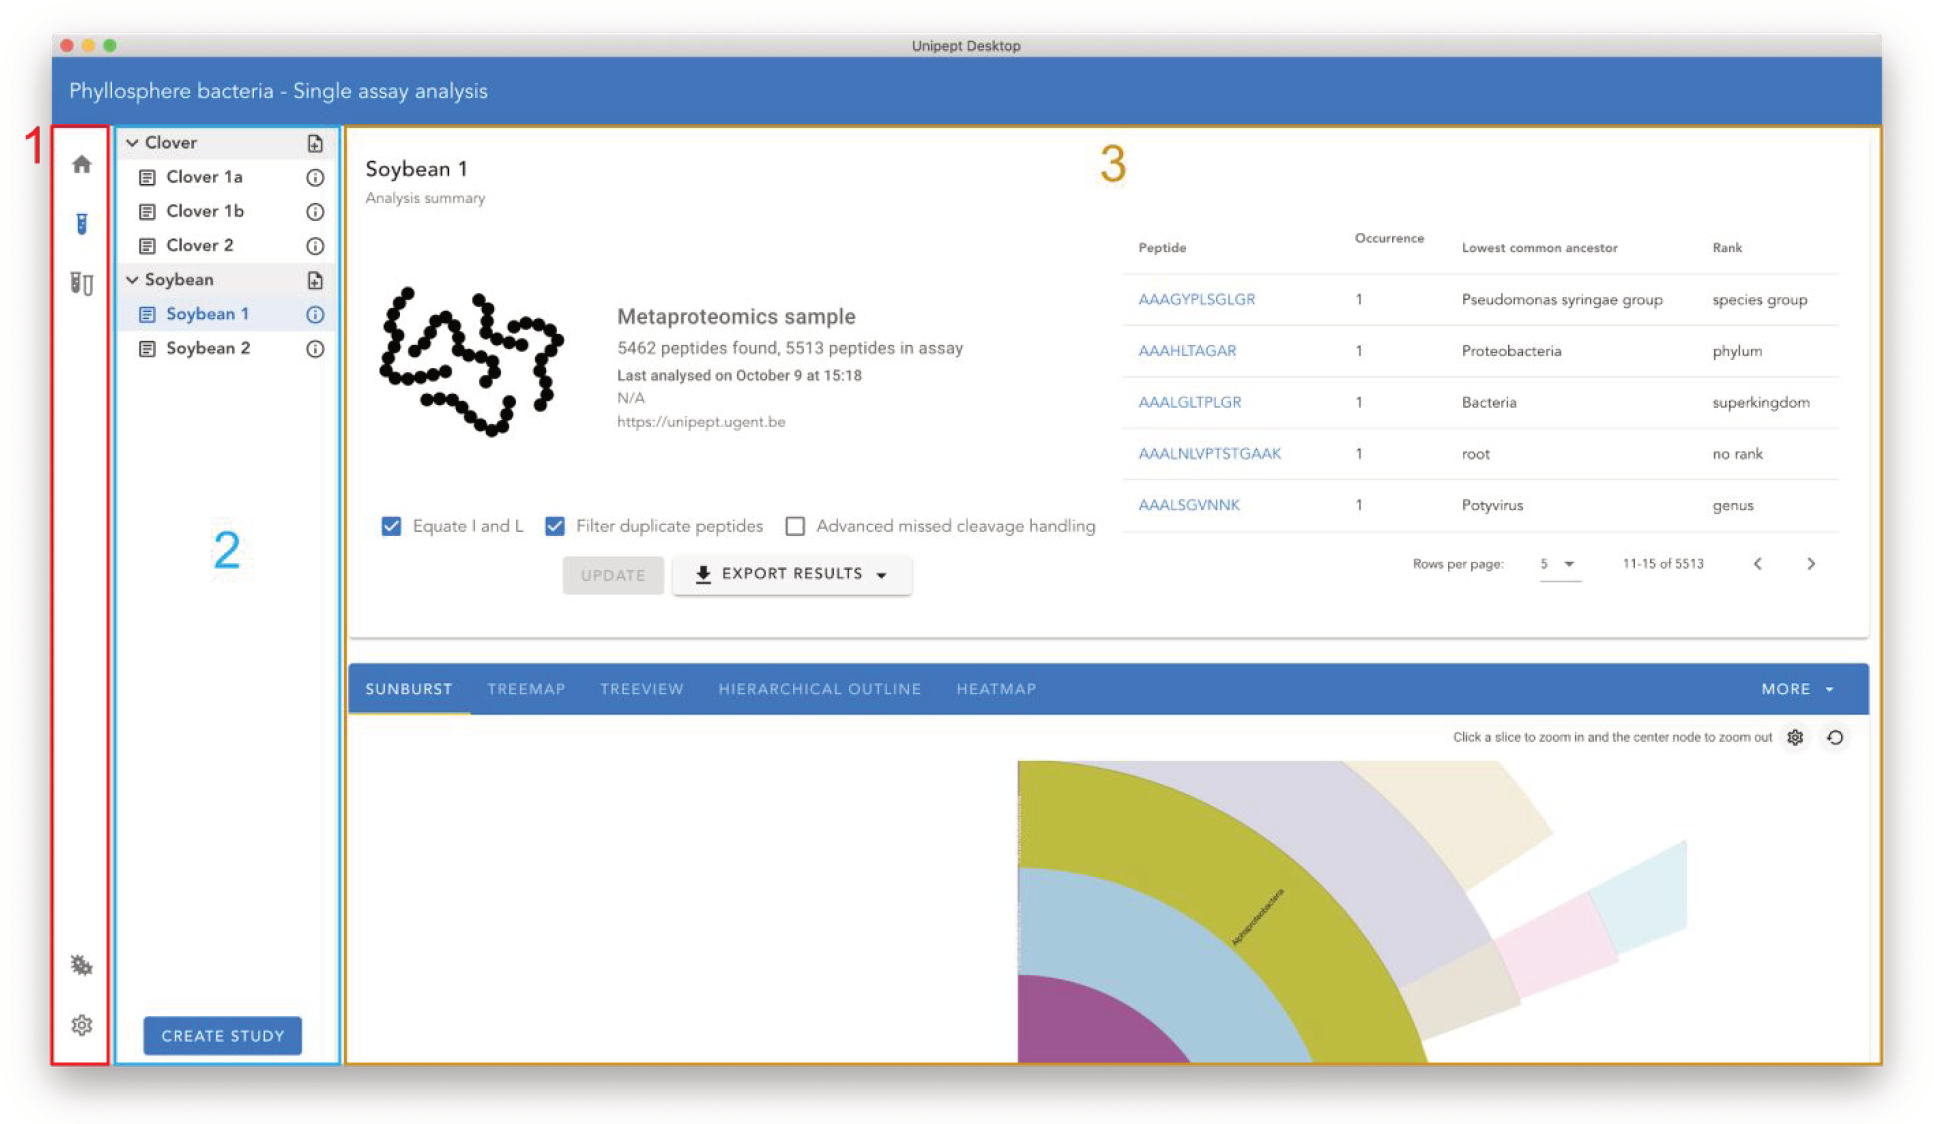
\includegraphics{resources/figures/chapter2_application_overview_screenshot.png}
\caption{Screenshot of the Unipept Desktop application. The analysis
page of the desktop application is depicted here and consists of three
main parts: the sidebar that is used to navigate between the different
analysis pipelines and functions of the application (1), the project
explorer that displays a hierarchical view of the project (2) and the
content view that renders analysis results (3).}
\end{figure}

The Unipept desktop application provides three different types of
analyses: \emph{i}) single assay analysis, \emph{ii}) inter-assay
comparative analysis, and \emph{iii}) tryptic peptide analysis. The
single assay analysis performs a full taxonomic and functional analysis
of a single assay and corresponds to the default ``metaproteomics
analysis'' as presented by the Unipept web application. The inter-assay
comparative analysis on the other hand, provides the ability to explore
similarities and differences between multiple assays. While the
comparison of multiple assays was already possible with the Unipept web
application, this was only available for a limited number of quite small
assays due to strict memory constraints posed by web browsers. The
tryptic peptide analysis, lastly, can be used to look up which proteins,
taxa and functions are associated with a given peptide.

Unipept Desktop delivers these core functions through a concise user
interface (Figure 1) that consists of three main parts: the sidebar, the
project explorer, and the content view. The sidebar on the far left
allows the user to navigate between the different analysis pipelines and
functions of this application. Directly to the right of the sidebar is
the project explorer that allows the user to switch between assays, and
to modify the project. The project explorer is only shown when
performing single assay or comparative analyses. Assays and studies can
be renamed or deleted by right clicking them, after which a context menu
opens. Lastly, the content view takes up most of the application's
visual space and presents either analysis results or the settings page.

The Unipept Desktop Application also allows offline analysis of data
through a choice of the API endpoint in the settings menu. This
endpoint, which uses the Unipept API and by default connects to the
online Unipept system, can be configured to call any service that
supports the Unipept API. By setting up a local instance of the Unipept
backend system, the user can thus ensure that all data remains locally.
Setting up a local Unipept back-end is possible by cloning the open
source Unipept repository on GitHub, but requires advanced technical
knowledge. We plan to make the installation process of these custom API
endpoints even easier with future releases of Unipept.

Unipept Desktop is powered by the cross-platform Electron framework,
which in itself is powered by Chromium browser technology. This means
that the application is developed with web-centric technologies, such as
the Vue frontend framework and TypeScript, and hence we were able to
reuse large parts of the web app's codebase. The choice for the Electron
platform was mostly driven by the extensive suite of different
functionalities that can be integrated with minimum configuration
efforts. Thanks to the Electron platform we can provide an automatic
update mechanism, easily generate installation packages for all major
platforms (Windows, macOS and Linux), and include automatic crash
reporting, amongst others. Once installed, the Unipept Desktop
application can thus update fully autonomously in the background,
ensuring that users always have the latest functionality and bug fixes
installed.

\hypertarget{project-centric-analysis}{%
\subsection{Project-centric analysis}\label{project-centric-analysis}}

The Unipept Desktop Application has full access to the local filesystem.
Hence, it can store an arbitrary amount of data and does not need to
worry about strict size limits; this in contrast to web applications
that are only allowed to store up to a few megabytes using the local
storage API. This allows us to improve upon the organization of data
sets by introducing project-based data management capabilities. In
accordance with the terminology introduced by the ISA-tab standard for
experimental metadata annotation 12, we now refer to a data set derived
from a sample as an ``assay'', while a study is a grouping of multiple,
related assays, and a Unipept project represents a collection of such
studies.

On the file system, a project is stored in a single folder that contains
an SQLite database file, a subfolder for each study and one text file
per assay, located in the subfolder of the corresponding study. This
folder can be modified outside of the application, using the default
file explorer application of your operating system, thus providing
maximum flexibility. All changes made to this project folder are
automatically detected and imported by the application, granting users
the ability to mass import assays and edit project properties with
external applications. The application accepts simple text files with
one peptide per line. In order to quantify peptide occurrence, a peptide
can be included more than once in this file and the ``filter duplicate
peptides'' option should be disabled for the analysis.

Because projects are folder-based, they can contain both the raw input
data as well as the analysis results for an assay, making it practical
for users to share projects with each other, for instance, in the form
of compressed project folders. In addition, previously performed
analyses do not need to be recomputed when the application is restarted,
as opposed to analyses that were run on the Unipept website, which need
to be recomputed every time the web site is closed.

\hypertarget{comparative-analysis}{%
\subsection{Comparative analysis}\label{comparative-analysis}}

\begin{figure}
\centering
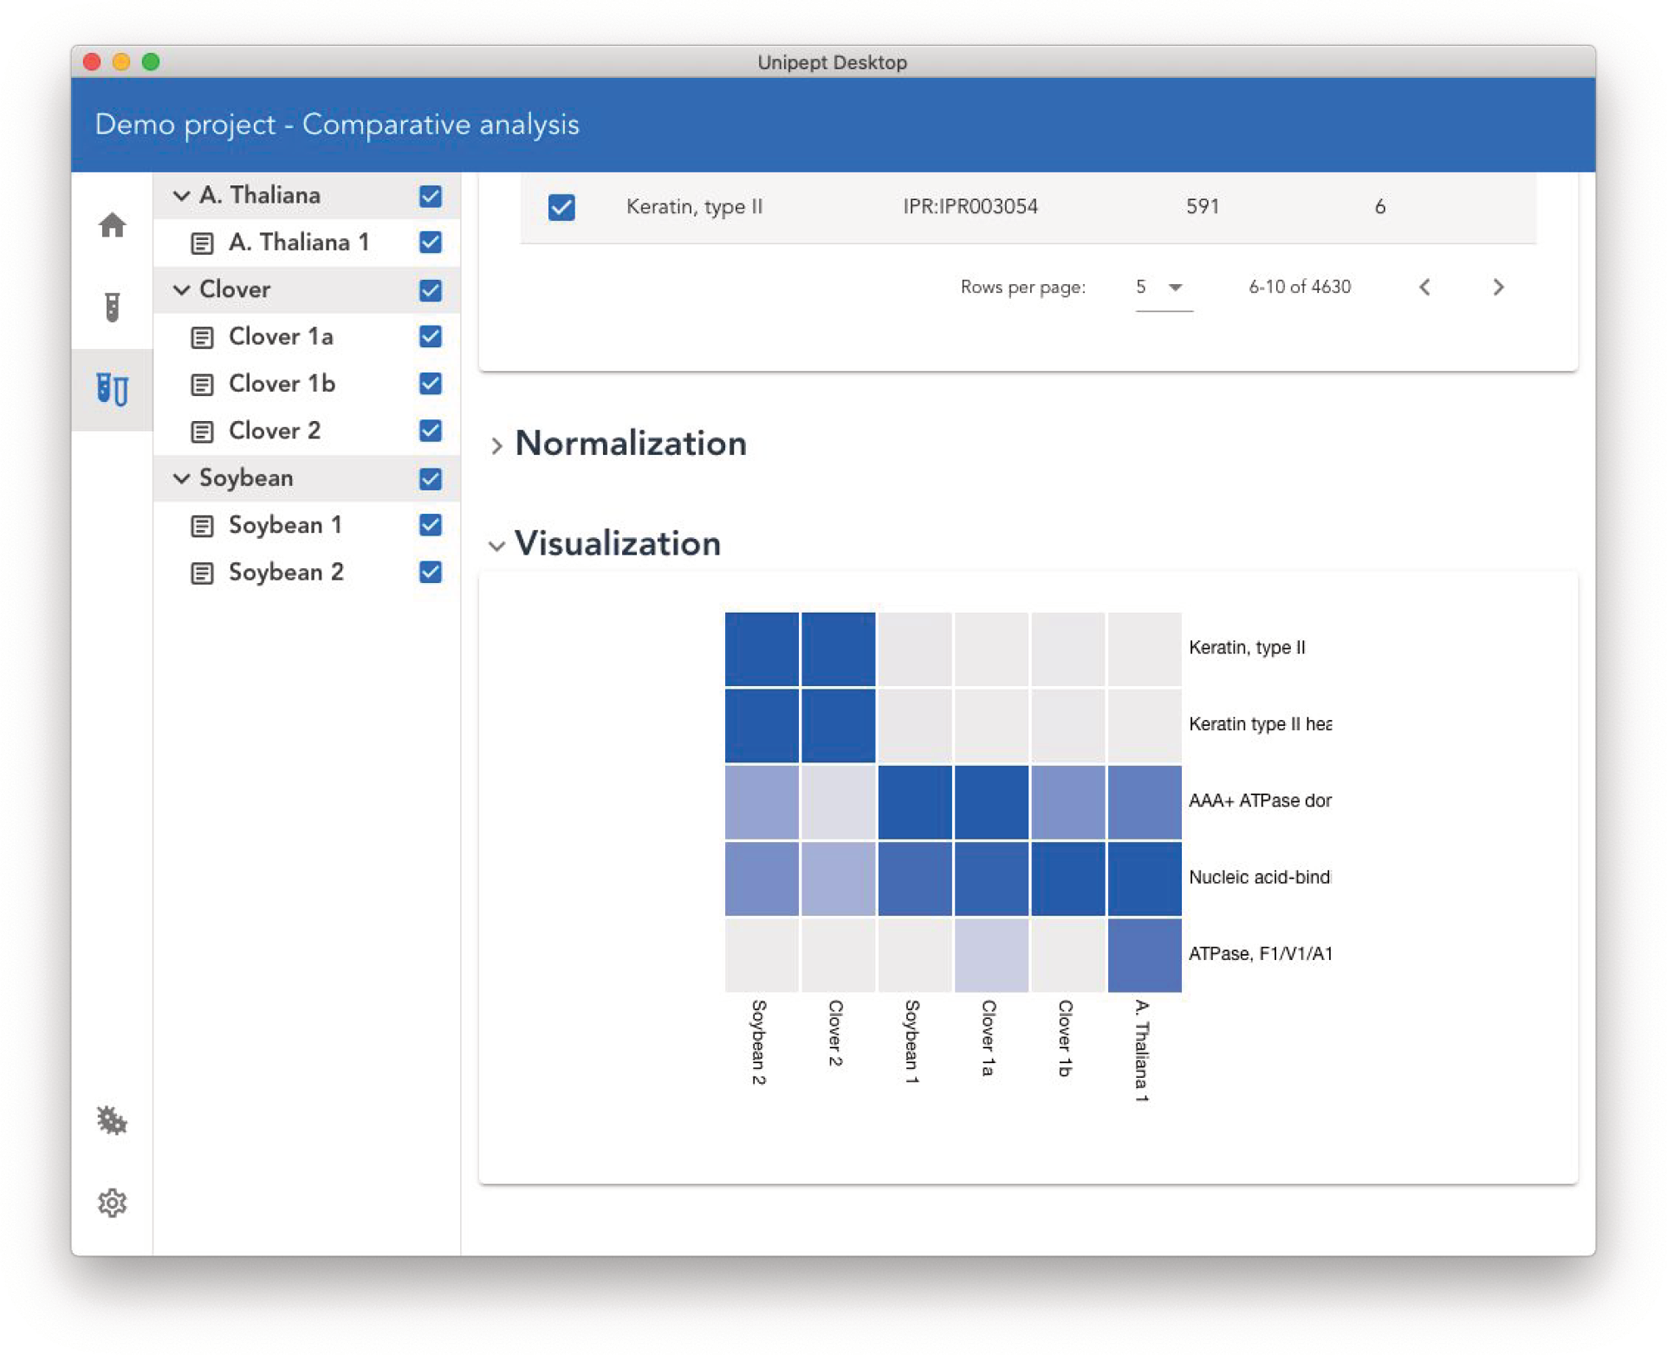
\includegraphics{resources/figures/chapter2_comparative_analysis_screenshot.png}
\caption{Screenshot of the inter-assay comparative analysis pipeline.
Note that it is possible to select multiple assays from the project
explorer. A heatmap is constructed from the set of items that were
selected for comparison at the top of the page.}
\end{figure}

The Unipept Desktop Application provides both intra-assay and
inter-assay comparative analyses that are rendered as heatmap
visualizations. The intra-assay comparison can be started from the
single assay analysis page by selecting the heatmap tab and provides a
wizard to guide users through the set-up process of the comparison
(Figure 2). Users are required to select two types of data sources (one
for each axis of the heatmap) and indicate which items should be
compared. Four different data sources are currently supported: NCBI
taxa, GO terms, EC numbers and InterPro entries.

The inter-assay comparative analysis is designed to visualize
differences and similarities in functional or taxonomic composition of
multiple assays. Here too, users are presented with a wizard that is
similar to the one found in the intra-assay comparison. For inter-assay
comparisons, however, the horizontal axis of the heatmap is reserved for
the set of selected assays, and users can therefore only select one
collection of items that should be compared between the different
assays.

Because the number of peptides can drastically differ between multiple
assays, three different normalization techniques are provided to the
user. The default setting normalizes the heatmap globally, i.e.~the
minimum and maximum values over the complete grid are computed and all
grid values are normalized with respect to these values. The other two
normalization techniques also normalize based on minimum and maximum
values, but restricted within a row or column, respectively.

It is worth noting that, while the comparative analysis pipeline was
originally designed for the Unipept Desktop Application, a slimmed-down
version has meanwhile also been integrated into the Unipept web app.

With the advent of the Unipept Desktop Application, users now have a
variety of ways in which they can use Unipept. A comparison between the
various functionalities offered by these different services is provided
in Table 1 below.

\hypertarget{conclusion}{%
\section{Conclusion}\label{conclusion}}

Unipept Desktop is a novel desktop application that extends upon the
Unipept web application by eradicating the strict limitations posed by
the web-based nature of this application to increase metaproteomics data
analysis throughput. Moreover, the Unipept Desktop Application adds new
features such as allowing users to structure their data in a
hierarchical project-based system, to keep track of their analysis
results, and to share or distribute these results very easily. Whereas
the Unipept web application is limited to assays with up to 50 000
peptides, the Unipept Desktop Application supports assays containing one
million peptides or more. For reference, the desktop app can analyze
between 250 and 2000 peptides per second (without advanced missed
cleavage handling enabled), depending on the type of assay that's being
analyzed.

In a future release of the Unipept Desktop Application, we plan to
provide support for the preparation of custom reference databases and
further improve support for offline analysis. This will allow us to
gradually evolve to a tool that is not only suitable for metaproteomics
data analysis, but also for novel proteogenomics analysis techniques for
complex environmental samples.

Our choice for the Electron framework proves to be very valuable as
well, as a large portion of Unipept's codebase can thus be shared
between the new desktop application and the existing web application.
This in turn allows us to easily migrate (a slimmed-down version of)
specific desktop features to the web app, and vice versa.

\hypertarget{availability}{%
\section{Availability}\label{availability}}

The source code for Unipept Desktop is open source and provided under
the MIT license as a repository on GitHub:
\url{https://github.com/unipept/unipept-desktop}. Pre-generated
installers for Windows, macOS and Linux (AppImage format) can be
downloaded from the release page of our GitHub repository. Installation
instructions and documentation for the Unipept Desktop Application can
be found on our website: \url{https://unipept.ugent.be/desktop}.

\hypertarget{acknowledgements-1}{%
\section{Acknowledgements}\label{acknowledgements-1}}

This work was supported by the Research Foundation---Flanders (FWO)
{[}1164420N to P.V.; 12I5220N to B.M.; 1S90918N to T.V.D.B.; G042518N to
L.M. {]}.
